\chapter{Los prototipos y el interfaz piDA.}
\epigraphhead [30]{%
  \epigraph{``Hoy en día la mayoría del software existe no para resolver un problema, sino para actuar de interfaz con otro software"}%
  {Ian O. Angell, profesor.}%
}

	En este capítulo se explican los dos prototipos desarrollados en el proyecto paralelo y su integración en nuestro programa junto con el interfaz piDA.
	
		\section{El interfaz piDA.}
		Para operar con los prototipos se ha desarrollado junto a los mismos la librería bautizada como piDA\footnote{Se puede encontrar en el siguiente repositorio git: \url{http://github.com/noeldiazro/piDA}} que implementa el diseño detallado en la \autoref{subsec:especificacion_piDA}.
		
		En lugar de empotrar la librería en el programa y hacerlos una sola entidad, se ha decidido que tanto la librería como el programa sigan siendo dos elementos independientes. De este modo ambos proyectos pueden seguir mejorando por separado y las mejoras implementadas en uno u otro no necesitan una nueva integración en el código, sino que son totalmente actualizables por separado gracias a github.
		
		Además, se incluye un instalador con la librería que configura la Raspberry Pi, instala las dependencias de piDA y deja el sistema preparado para funcionar con los prototipos.


	\section{El primer prototipo.}\label{sec:primer_prototipo}
			\begin{figure}[H]
			\centering
		  	\includegraphics[width=1\textwidth]{img/proto1.png}
  			\caption{El primer prototipo conectado a la Raspberry Pi.}\label{fig:proto1}
		\end{figure}
		El primer prototipo (\autoref{fig:proto1}) cuenta con un chip convertidor analógico/digital MCP3202 que provee dos entradas analógicas y precisión de 12 bits. El chip se comunica con la Raspberry Pi a través de un interfaz de serie compatible con el protocolo SPI, la conexión con la misma es mediante los pines GPIO. Podemos controlar la tensión que lee el chip mediante dos potenciómetros conectados a sendos canales. Todo el conjunto está montado sobre una placa de prototipado o \emph{protoboard}.
		Los datos que se obtienen del mismo son voltios, concretamente entre 0 y 3,3 ya que la misma placa se alimenta de la propia Raspberry, no requiriendo así alimentación externa. Durante el desarrollo de los siguientes prototipos esto cambiará para poder conectar los sensores del interfaz original PASCO (éstos operan entre $ \pm 10 $voltios y algunos requieren alimentación extra de 5 y/o 12 voltios). 
		

	\subsection{Implementación en el programa.}
		Se ha decidido realizar la implementación de la librería directamente y prescindir de la portabilidad del programa a otros sistemas operativos dejando esta característica como una futura mejora. Al ser una librería de Python mas, con solo importarla en nuestro programa ya tenemos acceso a sus módulos, especialmente al módulo Acquisition, que es nuestro nexo de conexión.
		
		Al disponer solo de dos canales disponibles según el prototipo pero tener el interfaz gráfico preparado para cuatro canales y no tener ninguna manera de obtener a través de la librería el número de canales ofrecidos, se ha programado de manera que la interfaz gráfica intenta inicializar cada uno de los cuatro canales y si alguno falla simplemente queda marcado como ``no disponible'' y se desactivan los controles asociados al mismo en el interfaz gráfico. 
		
		\subsection{Utilización del prototipo.}
		La librería se comportó según lo acordado en el diseño, por tanto tras la integración de ésta el funcionamiento fue el esperado y los cambios en el código original fueron mínimos. En la \autoref{fig:pida_2ch_sample} se puede ver un ejemplo de su funcionamiento.
		
	\begin{figure}[H]
			\centering
		  	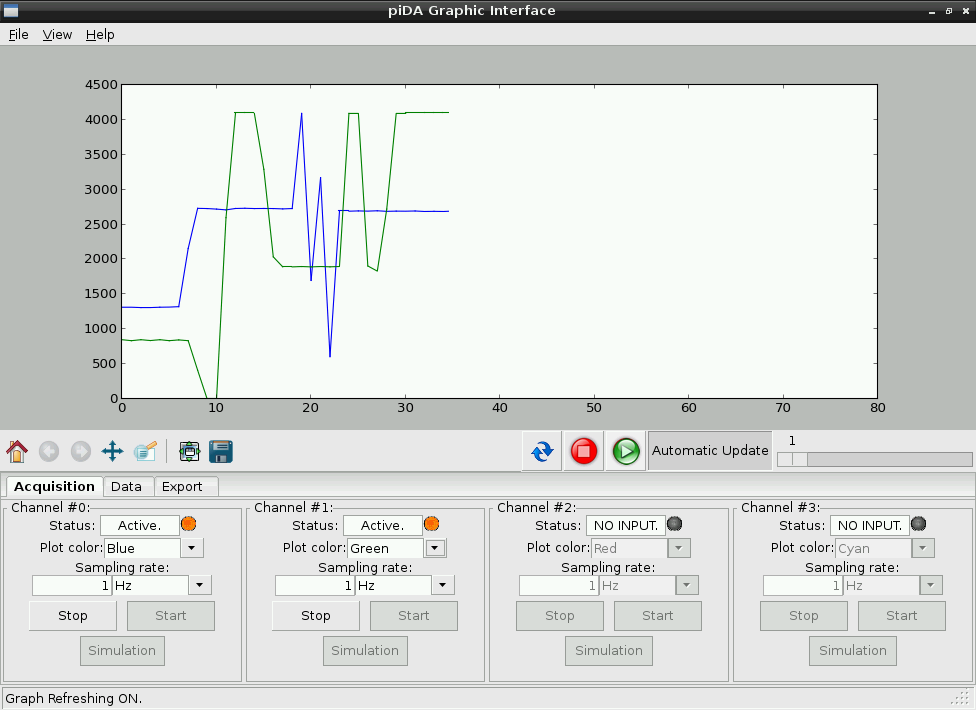
\includegraphics[width=1\textwidth]{img/pida_2ch_sample.png}
  			\caption{Funcionamiento del primer prototipo de dos canales.}\label{fig:pida_2ch_sample}
		\end{figure}
		\section{Segundo prototipo.}
			\begin{figure}[H]
			\centering
		  	\includegraphics[width=1\textwidth]{img/proto2.png}
  			\caption{El segundo prototipo conectado a la Raspberry Pi.}\label{fig:proto2}
		\end{figure}
		El segundo prototipo (\autoref{fig:proto2}) cuenta con las mismas características que el primero pero esta vez con dos chips MCP3202 dando soporte para cuatro canales. Dos de ellos son sensores: uno de luz y otro de temperatura. La distribución de canales por tanto es la siguiente:
		\begin{itemize}
			\item Canal 0: Potenciómetro (azul).
			\item Canal 1: Sensor de temperatura
			\item Canal 2: Sensor de luz.
			\item Canal 3: Potenciómetro (negro).
		\end{itemize}

		Los sensores no se han calibrado por lo que los datos obtenidos de ellos siguen siendo voltaje entre 0 y 3,3 voltios.
		
		\subsection{Implementación y utilización en el programa.}
		El código estaba preparado para ser utilizado hasta con cuatro canales, por tanto no hizo falta acondicionar nada del mismo para la conexión del nuevo prototipo.
		
		El funcionamiento una vez más fue el esperado, recibiendo datos de los cuatro canales y toda la mecánica funcionando sin ningún problema, incluída la visualización y exportación de los datos. 
		En la \autoref{fig:pida42ch_sample} se puede ver una captura del programa funcionando a distintas frecuencias e interactuando con los distintos canales.
		
			\begin{figure}[H]
			\centering
		  	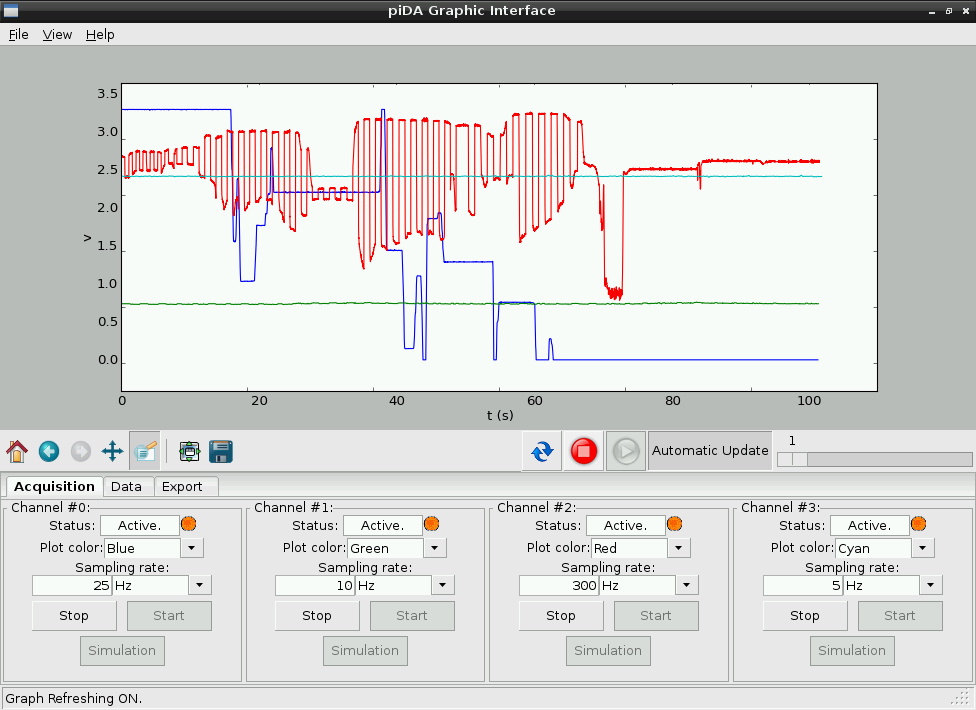
\includegraphics[width=1\textwidth]{img/pida_4ch_sample.png}
  			\caption{Funcionamiento del segundo prototipo con cuatro canales.}\label{fig:pida42ch_sample}
		\end{figure}